\chapter{Optimeringsmetoder} \label{kap:optimeringsmetoder}
\textit{Lasso problemet er et quadratic programming problem med lineære uligheder. 
Flere algoritmer kan løse dette problemet grundet konveksiteten.  
I dette kapitel beskrives to af disse algoritmer kaldet coordinate descent og Least Angle Regression (LARS).} \\[4mm]
%
For en model matrix i general position (se definition \ref{defn:general_position}) findes der ikke en eksplicit løsning for lasso estimatoren.
Men som sagt er objektfunktionen af lasso problemet \eqref{eq:2.5} konveks.
For at vise dette kan objektfunktionen skrives som
\begin{align*}
f \del{\beta} = g \del{\beta} + h \del{\beta},
\end{align*}
hvor \(g \del{\beta} = \Vert \y - \X \beta \Vert_2^2\) og \(h \del{\beta} = \lambda \Vert \beta \Vert_1\).
For \(g \del{\beta}\) udregnes Hessematricen
\begin{align*}
\Delta^2 g \del{\beta} = \frac{\partial^2 g }{\partial \beta_i \partial \beta_j} = 2 \X^T \X.
\end{align*}
For enhver vektor \(\ell \in \R^p\) er \(\ell^T \X^T \X \ell > 0\), dvs \(\ell^T \X^T \X \ell \) er positiv semidefinit, hvilket medfører at \(g \del{\beta}\) er konveks.
For ethvert \(\alpha \in \del{0,1}\) og \(\beta\), \(\beta'\) har vi at
\begin{align*}
h \del{\alpha \beta + \del{1+\alpha}\beta'} &= \lambda \Vert \alpha \beta + \del{1+\alpha} \beta' \Vert_1 \\
&\leq \lambda \Vert \alpha \beta \Vert_1 + \lambda \Vert \del{1+\alpha} \beta' \Vert_1 \\
&= \lambda \alpha \Vert \beta \Vert_1 + \lambda \del{1+\alpha} \Vert \beta' \Vert_1 \\
&= \alpha h \del{\beta} + \del{1+\alpha} h \del{\beta'},
\end{align*}
hvilket medfører, at \(h \del{\beta}\) er konveks af definition \ref{defn:konveks}.
Da summen af to konvekse funktioner er konveks, medfører dette konveksiteten af \(f \del{\beta}\). 

Som nævnt i underafsnittet \ref{subsec:udregning_lasso} er \(\ell_1\)-normen \(\sum_{j=1}^p \vert \beta_j \vert\) ikke differentialbel i \(\beta = 0\).
En general egenskab af differentialble konvekse funktioner er, at en første ordens tangent approksimation altid giver en nedre grænse.
Begrebet subgradient er baseret på en generalisering af dette.
Givet en konveks funktion \(f: \ \R^p \rightarrow \R\), siges \(z \in \R^p\) at være en subgradient af \(f\) i \(\beta\) hvis
\begin{align*}
f \del{\beta'} \geq f \del{\beta} + \left\langle z, \beta' - \beta \right\rangle, 
\end{align*}
for alle \(\beta' \in \R^p\).
Geometrisk er subgradient vektoren \(z\) normal til et hyperplan som understøtter ---.
Mængden af alle subgradienter af \(f\) i \(\beta\) kaldes \textit{subdifferential} og betegnes \(\partial f \del{\beta}\).
Når \(f\) er differentialble i \(\beta\), da reduceres subdifferentialet til én vektor, givet ved \(\partial f \del{\beta} = \cbr{\nabla f \del{\beta}}\).
I punkter hvor \(f\) ikke er differentialble, da er subdifferentialet en konveks mængde bestående af alle mulige subgradienter.




\section{Coordinate descent} \label{sec:theory_coordinatedescent}
%Ideen bag coordinat descent er, at optimere en target funktion mht én parameter mens de resterende parametre fastholdes. 
%Vi gennemløber alle parametre iterativ indtil konvergens.
%Coordinate descent er specielt attraktiv for problemer som lasso, som har en simpel lukket løsning for en dimension, men ikke for flere dimensioner.
%
Coordinate descent er en iterativ algoritme, som opdaterer fra \(\tbeta^t\) til \(\tbeta^{t+1}\) ved at vælge én koordinat som opdateres, og da udføres en univariat minimering over denne koordinat.
Hvis koordinat $k$ er valgt i iteration $t$, da er opdateringen givet ved
\begin{align}
\beta_k^{t+1} =\underset{ \beta_k}{\arg \min}  f\del{ \beta_1^t, \beta_2^t, \dots, \beta_{k-1}^t, \beta_k, \beta_{k+1}^t, \dots, \beta_p^t  }, \label{eq:5.36}
\end{align}
hvor $\beta_j^{t+1} = \beta_j^t$ for $j \neq k$. 
Typisk gennemløbes koordinaterne i en forudbestemt rækkefølge.
Dette kan generaliseres til \textit{block coordinate descent}, som anvendes for group lasso, hvor prædiktorerne er opdelt i ikke-overlappende blocks, og da udføres en minimering over en enkelt block for hvert koordinat.

For at algoritmen konvergerer til det globale minimum af en konveks funktion, skal funktionen være kontinuert differentiabel og strengt konveks i hver koordinat. 
Men som nævnt er strafleddet for lasso ikke differentiabel.

For mange optimeringsproblemer kan objektfunktionen dekomponeres
\begin{align}
f(\beta_1, \dots, \beta_p) = g(\beta_1, \dots, \beta_p) + \sum_{j = 1}^p h_j \del{\beta_j}, \label{eq:5.37}
\end{align}
hvor \(g: \R^p \rightarrow \R\) er differentiabel og konveks og \(h_j: \R \rightarrow \R\) er konveks, men ikke nødvendigvis differentiabel.
Bemærk at lasso problemet \eqref{eq:2.5} kan dekomponeres som \eqref{eq:5.37} med \(g \del{\tbeta} =\Vert \y - \X \tbeta \Vert_2^2\) og \(h_j \del{\beta_j} = \lambda \vert \beta_j \vert\).
\citep{Tseng_coordinate} viste, at for enhver konveks funktion \(f\) som kan opdeles som \eqref{eq:5.37}, vil coordinate descent algoritmen \eqref{eq:5.36} konvergere til det globale minimum. 
Nøgleegenskaben bag dette resultat er, at den ikke-differentiable komponent \(h \del{\beta} = \sum_{j=1}^p h_j \del{\beta_j}\), kan opsplittes som summen af funktioner af hver individuel parameter.
Resultatet betyder, at coordinate descent kan bruges til at løse lasso og dens generaliseringer, som beskrives senere i specialet.
Hvis den ikke-differentiable komponent \(h\) ikke kan opsplittes, da kan det ikke garanteres at coordinate descent konvergerer.

%\subsubsection{Lineær regression og lasso}
%Optimalitets betingelserne for lasso problemet \eqref{eq:2.5} er
%\begin{align*}
%-2 \sum_{i=1}^n \del{y_i - \sum_{k=1}^p x_{ik} \beta_k} x_{ij} + \lambda s_j = 0,
%\end{align*}
%hvor \(s_j =\text{sign} \del{\beta_j^*}\) hvis \(\beta_j^* \neq 0\) og \(s_j \in \sbr{-1,1}\) hvis \(\beta_j^* = 0\) for \(j=1, \ldots, p\).
%Coordinate descent algoritmen løser disse ligninger og itererer over \(j=1,2,\ldots,p,1,2, \ldots\).
%Lad os definer det partielle residual \(r_i^{(j)} = y_i - \sum_{k \neq j} x_{ik} \widehat{\beta}_k\), som fjerner nuværende fit fra alle undtaget \(j\)'te prædiktor.
%Da er opdateringen givet ved
%\begin{align*}
%\widehat{\beta}_j = S_\lambda \del{\tilde{\beta}_j},
%\end{align*}
%hvor \(\tilde{\beta}_j\) er koefficienten af en simpel lineær regression af det partial residual på variabel \(j\).
\newpage
\begin{alg} [Coordinate descent for lasso problemet]
\begin{enumerate}
\item Standardisér prædiktorerne \(\x_1, \ldots, \x_p\) og centrér responsvariablen.
Definer en følge af værdier \(\lambda_0 > \lambda_1 > \ldots > \lambda_L\), hvor \(\lambda_0\) vælges, således at \(\widehat{\tbeta}^\text{lasso} \del{\lambda_0} =\mathbf{0}\).
\item For hvert \(\lambda \in \cbr{\lambda_0, \ldots, \lambda_L}\), gentages følgende trin for \(j = 1, \ldots, p\) indtil konvergens:
\begin{itemize}
\item Opskriv lasso problemet \eqref{eq:2.5}
\begin{align*}
\sum_{i=1}^n \del{y_i - \sum_{k \neq j} x_{ik} \widehat{\beta}^\text{lasso}_k - x_{ij} \beta_j}^2 + \lambda \sum_{j = 1}^p \vert \beta_j \vert,
\end{align*}
hvor \(\widehat{\beta}^\text{lasso}_k \del{\lambda}\) er det nuværende estimat for \(\beta_k\) for et given \(\lambda\), hvor \(k \neq j\).
\item Udregn de partielle residualer: \(r_{i}^{(j)} = y_i - \sum_{k \neq j} x_{ik} \widehat{\beta}^\text{lasso}_k \del{\lambda}\) for alle \(i\)
\item Udregn koefficienten af en simpel lineær regression af den partielle residual på \(j\)'te prædiktor: \(\tilde{\beta}_j = \frac{1}{n} \sum_{i=1}^n r_{i}^{(j)} x_{ij}\) 
\item Opdater det nuværende estimat \(\widehat{\beta}^\text{lasso}_j\) ud fra soft-thresholding operatoren
\begin{align}
\widehat{\beta}^\text{lasso}_j \del{\lambda}= S_{\frac{\lambda}{2n}} \del{\tilde{\beta}_j}. \label{eq:update_coordinate}
\end{align}
\end{itemize}
\end{enumerate}
\end{alg}
%
Løsningerne udregnes for en aftagende følge af værdier \(\cbr{\lambda_{\ell}}_{\ell = 0}^L\), hvor \(\lambda_0\) vælges således at \(\widehat{\tbeta} \del{\lambda_0} =\mathbf{0}\). 
Algoritmen udnytter \textit{warm start}, hvilket betyder, at \(\widehat{\tbeta} \del{\lambda_\ell}\) anvendes som begyndelsesværdi for løsningen \(\widehat{\tbeta} \del{\lambda_{\ell + 1}}\), dette fører til en mere stabil algoritme. 
Når \(\widehat{\tbeta} = \mathbf{0}\), har vi, at \(\widehat{\beta}_j\) vil forblive nul hvis \(\frac{1}{n} \left\vert \left\langle \mathbf{x}_j, \mathbf{y} \right\rangle \right\vert < \frac{\lambda}{2n}\). Derfor er \( \lambda_0 = 2 \max_j \left\vert \left\langle \mathbf{x}_j, \mathbf{y} \right\rangle \right\vert\).
Strategien er at vælge en minimum værdi \(\lambda_L = \epsilon \lambda_0\) og konstruere en følge af \(K\) værdier af \(\lambda\), som aftager fra \(\lambda_0\) til \(\lambda_L\) på logskalaen.
Typiske værdier er \(\epsilon = 0.001\) og \(K =100\).

Den beskrevne coordinate descent algoritme er implementeret i \Rlang-pakken \texttt{glmnet}.
Koefficientstierne i figur \ref{fig:diabetes_koef} er fundet ud fra denne algoritme.

\section{LARS}
LARS algoritmen var først introduceret i \citep{efron}.  
Vi introducerer først den originale version af LARS algoritmen, hvor efter vi laver en simple modifikation af LARS algoritmen for at løse lasso. 

Ideen bag algoritmen er, at vi først sætter alle koefficienter lig nul, hvor vi herefter finder den , $x_{1j}$, som er mest korrelerede med respons variablen, $\textbf{y}$.  
Vi tager hernæst den størst mulige trin i retningen af vores prædiktor, hvor vi anvender en simple lineær regression af $\textbf{y}$ på $x_{1j}$. 
Vi får en residual vektor, som er ortogonal på $x_{j1}$ og bliver vores nye respons. 
Vi fortsætter indtil $x_{2j}$ er lige så korrelerede  med residualerne, som $x_{j1}$. 
LARS algoritmen anvender herefter den ensvinklet retning mellem $x_{1j}$ og $x_{2j}$, som den nye retning indtil den rammer den tredje variable, som er den mest korrelerede, hvorefter den nye retning er ensvinklet mellem de de tre variable $x_{1j}$, $x_{2j}$ og $x_{3j}$. Dette fortsættes. 

I hvert trin bliver der tilføjet en kovariat til vores model $\widehat{\boldsymbol{\mu}} = \textbf{X} \widehat{\boldsymbol{ \beta}}$, så efter $k$ iterationer er der k elementer i  $\widehat{\beta}_j$, som er forskellige fra nul.  

Figur \ref{fig:lars} illustrerer algoritmen, hvor $p = 2$ og $X = \del{\textbf{x}_1, \textbf{x}_2}$. 
Vi lader kovariaterne være standardiseret med middelværdi 0 og unit varians og lader respons have en middelværdi 0. Den nuværende korrelation er givet ved 
\begin{align*}
\textbf{c}\del{\boldsymbol{\widehat{\mu}}} = X^T\del{\textbf{y} - \widehat{\boldsymbol{\mu}}} = X^T \del{ \textbf{y}_2 - \boldsymbol{\widehat{\mu}}}.
\end{align*}
I dette tilfælde er den nuværende korrelation kun afhængige af projektionen $\textbf{y}_2 $, som er projektionen af $\textbf{y}$ i det lineære rum $L(X)$ udspændt af $ \textbf{x}_1 $og $\textbf{x}_2$. 
Algoritmen starter i $\widehat{\boldsymbol{\mu}}_0 = \textbf{0}$, hvor vi ser på figur \ref{fig:lars} at $ \textbf{y}_2 - \boldsymbol{\widehat{\mu}}_0$ og $\textbf{x}_1$ har den mindste vinkel i forhold til $ \textbf{y}_2 - \boldsymbol{\widehat{\mu}}_0$  og $\textbf{x}_2$, dvs at $\textbf{c}_1\del{\boldsymbol{\widehat{\mu}}_0} > \textbf{c}_2\del{\boldsymbol{\widehat{\mu}}_0}$. 
LARS algoritmen forstærker  $\boldsymbol{\widehat{\mu}}_0$ i retning af $\textbf{x}_1$ ved
%
 \begin{align*}
 \boldsymbol{\widehat{\mu}}_1 = \boldsymbol{\widehat{\mu}}_0 + \widehat{\gamma}_1 \textbf{x}_1.
 \end{align*}
 %
 Lad $\widehat{\gamma}$ være stepsize og bestemmes  således at $ \textbf{y}_2 - \boldsymbol{\widehat{\mu}}$ er lige korrelerede med $\textbf{x}_1$ og $\textbf{x}_2$, dvs det er når  $\textbf{y}_2 - \boldsymbol{\widehat{\mu}}_1$ deler vinkel i lige står dele mellem  $\textbf{x}_1$ og $\textbf{x}_2$, således at $\textbf{c}_1\del{\boldsymbol{\widehat{\mu}}_1} = \textbf{c}_2\del{\boldsymbol{\widehat{\mu}}_1}$.  
 
 Vi lader $\boldsymbol{\mu}_2$ være en enheds vektor liggende på bisektoren. Den næste LARS estimat er 
 %
 \begin{align*}
 \boldsymbol{\widehat{\mu}}_2 = \boldsymbol{\widehat{\mu}}_1+ \widehat{\gamma}_2 \boldsymbol{\widehat{\mu}}_2,
 \end{align*}
%
hvor $\widehat{\gamma}_2$ er valgt således at  $ \boldsymbol{\widehat{\mu}}_2 = \textbf{y}_2$ i tilfældet hvor $p = 2$. 
%
\begin{figure}[H]
\centering
\scalebox{0.8}{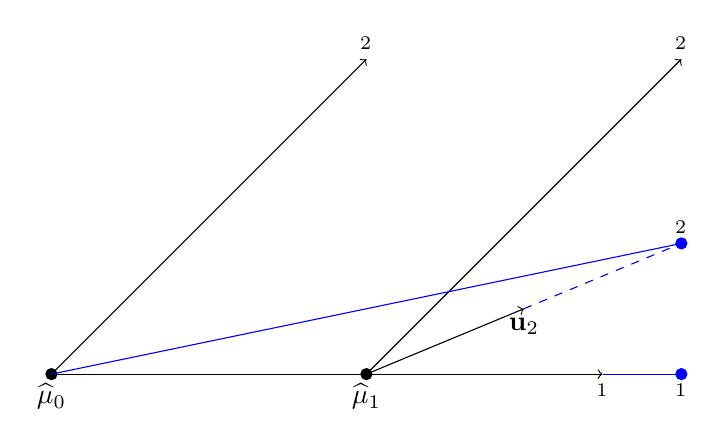
\begin{tikzpicture}
\draw [<-] (4,0) node [below] {$\x_1$}-- (-3,0);
\filldraw (1,0) circle (2pt) node [below] {$\widehat{\boldsymbol{\mu}}_1$};
\filldraw (-3,0)  circle (2pt) node [below]{$\widehat{\boldsymbol{\mu}}_0$};
\draw [<-] (5,4) node [above] {$\x_2$} --(1,0);
\draw [<-] (1,4) node [above] {$\x_2$} --(-3,0);

\draw [blue](5,1.66)  node [above, black] {$\y_2$} -- (-3,0);

\draw [->](1,0) -- (3, 0.83)  node [below] {$\mathbf{u}_2$} ;
\draw [dashed, blue] (3,0.83) -- (5,1.66) ; 


\filldraw [blue] (5,1.66) circle (2pt) ;
\draw [blue]  (5,0) node [below] {} -- (4,0);
\filldraw [blue] (5,0) circle (2pt) ;
\draw (5,0) node [black, below] {$\y_1$};
\end{tikzpicture}}
\caption{Figuren viser LARS algoritmen, i tilfældet hvor $p = 2$. Vi har to kovariater  $\textbf{x}_1$ og $\textbf{x}_2$, $\textbf{y}_2$ er projektionen af $\textbf{y}$ in i det lineære rum $L  \del{ \textbf{x}_1, \textbf{x}_2} $. }\label{fig:lars}
\end{figure}
%
Vi vil beskrive algoritmen mere generelt.
Vi antager at kovariaterne $ \textbf{x}_1,  \textbf{x}_2,  \dots,  \textbf{x}_p$ er lineært uafhængige og lader $\mathcal{A}$ være en delmængde af indekser $\{1, 2, \dots, p \}$. 
Vi definerer følgende mængder 
%
\begin{align*}
X_{\mathcal{A}} & = \del{\cdots s_j \textbf{x}_j \cdots}  \nonumber \\ 
N_{\mathcal{A}} & = X^T_{\mathcal{A}} X_{\mathcal{A}} \\ \
A_{\mathcal{A}} & = \del{ \textbf{1}^T_{\mathcal{A}} N_{\mathcal{A}} \textbf{1}_{\mathcal{A}} }^{- 1/2} , \nonumber 
\end{align*}
%
hvor  $s_j = \pm 1$ og $\textbf{1}_{\mathcal{A}} $ er en vektor bestående af 1-taller, som har samme længde som $\abs{\mathcal{A}}$. 
Lad 
%
\begin{align*}
\textbf{u}_{\mathcal{A}} = X_{\mathcal{A}} \omega_{\mathcal{A}}, 
\end{align*}
%
kaldes den ensvinklet vektor og hvor $ \omega_{\mathcal{A}} = A_{\mathcal{A}} G^{-1}_{\mathcal{A}}  \textbf{1}^T_{\mathcal{A}}$. 

Der gælder følgende 
%
 \begin{align*}
 X^T_{\mathcal{A}} \textbf{u}_{\mathcal{A}} = A_{\mathcal{A}}  \textbf{1}_{\mathcal{A}}   \quad  \text{og} \quad \norm{ \textbf{u}_{\mathcal{A}}}^2 = 1.
\end{align*}  
%
Derudover lad $\widehat{c}$ være en vektor af nuværende korrelationer, lad $\widehat{C}$ være den maksimale nuværende absolut korrelation, og lad $s_j$ være fortegnet af $\widehat{c}$: 
%
\begin{align*}
 \widehat{\textbf{c}} & = X^T \del{ \textbf{y}- \widehat{\boldsymbol{\mu}}}, \\
 \widehat{C} & = \max_j \cbr{\abs{\widehat{c}_j}}, \\
 s_j &  = \text{sign} \cbr{\widehat{c}_j}, \quad \text{for } j \in \mathcal{A},
\end{align*}
%
hvor $\widehat{\boldsymbol{\mu}} = X \widehat{\beta}$ er det nuværende LARS estimat. Vi definerer den aktive mængde $\mathcal{A}$, som en mængde af indekser som tilhører de kovariater, som har den maksimale nuværende absolut korrelation med de nuværende remanens (residuum?).  Dvs 
\begin{align*}
\mathcal{A} = \cbr{j : \abs{\widehat{c}_j} = \widehat{C}} = \cbr{j : \widehat{\beta}_j \neq 0},
\end{align*}

\begin{alg} [LARS algoritmen]
\begin{enumerate}
%
\item Standardiserer prædiktorerne til at have en middelværdi 0 og $\norm{\textbf{x}_j}_2^2$ for alle $j$.
Vi starter med $\widehat{\boldsymbol{\mu}}_0 = 0$, $\widehat{\boldsymbol{c}} = X^T \textbf{y}$ og $\widehat{\boldsymbol\beta}_0 = \del{0, \dots, 0}^T$
%
\item Find prædiktoren $\textbf{x}_j$ med den højest værdi af  $ \abs{\widehat{c}_j}$ og definer den aktive mængde $\mathcal{A} = \cbr{j}$. 
%
\item Gentag følgende indtil alle prædiktoreren fra den komplementærmængde $\mathcal{A}^C$ er indeholdt i det aktive mængde
%
\begin{itemize}
%
\item Udregn  $\widehat{\textbf{c}}$, $ \widehat{C} $, $ X_{\mathcal{A}}$,$ A_{\mathcal{A}}$,  $\textbf{u}_{\mathcal{A}}$ ud fra overstående formler og det indre produkt vektor
%
\begin{align*}
\textbf{a} = X^T \textbf{u}_{\mathcal{A}} = \del{a_1, \dots, a_p}^T
\end{align*}
%
\item Opdaterer $\widehat{\boldsymbol{\mu}}_{\mathcal{A}}$ ved
\begin{align}
\widehat{\boldsymbol{\mu}}_{\mathcal{A}} = \widehat{\boldsymbol{\mu}}_{\mathcal{A}} + \widehat\gamma \textbf{u}_{\mathcal{A}} \label{eq:u}
\end{align}
%
hvor
\begin{align}
\widehat\gamma = \underset{j \in \mathcal{A}^C}{\min^+} \cbr{ \frac{\widehat{C}- \widehat{c}_j}{A_\mathcal{A} - a_j} \frac{\widehat{C} + \widehat{c}_j}{A_\mathcal{A} + a_j}}, \label{eq:j_indeks}
\end{align}
hvor $\min^+$ betyder, at minimum kun er taget af positive komponenter for hvert valg af $j$. 
\item Mængden $\mathcal{A} = \mathcal{A} \cup \widehat{j}$, hvor $\widehat{j}$ er den maksimale indeks i \eqref{eq:j_indeks}. 
\end{itemize}
\end{enumerate}
\end{alg}
Overstående viser hvordan algoritmen bliver brugt. Men for lasso skal der bruges en lille modifikation. 
Vi lader $\widehat{\boldsymbol\beta} = \del{\widehat{\beta}_1, \dots, \widehat{\beta}_p }^T$ være en lasso løsning til $\widehat{\boldsymbol{\mu}} = X \widehat{\boldsymbol\beta}$. Der gælder at fortegnet af enhver estimerede koefficient $\beta_j$ må have samme fortegn som den nuværende korrelation $\widehat{c}_j = \textbf{x}_j \del{\textbf{y} - \widehat{\mu}}$, 
\begin{align*}
\text{sign} \del{\widehat{\beta}_j} = \text{sign} \del{\widehat{c}_j} = s_j
\end{align*}
...... (bevis) 

For at tage den her modifikation i betragtning tilføjer vi følgende i tredje trin. 
\begin{itemize}
\item Definerer p-vektoren $\widehat{\textbf{d}} = s_j \omega_{\mathcal{A}_j}$ for $j \in \mathcal{A}$ og er ellers nul. Hvor $ \omega_{\mathcal{A}_j}$ betegner j'te elementet af vektoren $\omega_{\mathcal{A}}$. 
\item For $j \in \mathcal{A}$ opdaterer vi 
\begin{align*}
\widehat{\beta}_j \del{\gamma} = \widehat{\beta}_j + \gamma \widehat{d}_j 
\end{align*}
\item Vi lader 
\begin{align*}
\gamma_j = - \frac{\widehat{\beta}_j}{\widehat{f}_j} \quad \text{og} \quad \tilde\gamma = \underset{y_j > 0}{\min} \cbr{\gamma_j}. 
\end{align*}
\item Hvis $\gamma = \tilde{\gamma}$, så træk det$ \tilde{j}$'te elemeent fra udregning af den næste ensvinklet retning, dvs 
\begin{align*}
\widehat{\boldsymbol\mu}_{\mathcal{A}_+} = \widehat{\boldsymbol\mu}_\mathcal{A} + \tilde{\gamma} \textbf{u}_\mathcal{A} \quad \text{og} \quad \mathcal{A_+} = \mathcal{A}- \cbr{\tilde{j}}
\end{align*}
udregnes i stedet for \eqref{eq:u}.
\end{itemize}

Flere beskrivelser af algoritmen kan findes i \citep{efron}. 
LARS har følgende fordele.
En af dem er, at den giver en ranking af prædiktorer når der bliver tilføjet andre prædiktorer, som ikke er tilfældet med hard treshold. 
En anden fordel er at algoritmen undgår streng korrelerede prædiktorer, hvis en af de korrelerede prædiktorer allerede er inkluderet, siden at den nye residual vil have lav korrelation med variabler, som er streng korrelerede variabler, som allerede er inkluderet. 
Derudover er LARS algoritmen ikke er 'greedy', som forward regression, fordi den udnytter en god retning til dens maksimum . 
LARS algortimen har også samme beregnings omkostninger, som en velkendt OLS \citep{hui_hastie}. 


